\section{CalibX标定系统}
CalibX标定系统由软件系统和硬件系统组成。
\subsection{硬件}
硬件系统如图\ref{moon2_device}所示。该硬件系统主要由机械臂、标定板、光源、计算机及显示器、供电系统等组成。
\begin{figure}[h]
	\centering
	\includegraphics[width=1\textwidth]{figure/target/moon2_device}
	\caption{CalibX硬件系统}
	\label{moon2_device}
\end{figure}
该系统具有如下优点:
\begin{itemize}
	\item 立体标定板,支持大FOV鱼眼相机、支持多相机,多相机之间可以无重叠视场
	\item 4向可调高亮高均匀光源,箱体内镜头处光源强度可达2000lux,降低相机曝光时间,减轻卷帘曝光影响
	\item 机械臂、滑台滑环组合,连续转动不绕线
\end{itemize}
一些标定样品如图\ref{fig:calibx}所示。
\begin{figure}
	\centering
	\begin{minipage}{0.45\linewidth}
		\centering
		\subfigure[标定手机]{\includegraphics[width=\linewidth,height=8cm]{figure/target/cellphone}}
		\label{fig:subcaption1}
	\end{minipage}\qquad
	\begin{minipage}{0.45\linewidth}
		\centering
		\subfigure[标定眼镜]{\includegraphics[width=\linewidth,height=8cm]{figure/target/ar_glass}}
		\label{fig:subcaption2}
	\end{minipage}
	\caption{CalibX标定系统标定产品样例}
	\label{fig:calibx}
\end{figure}
\subsection{软件}
软件系统如图\ref{fig:calibx_framework}所示。整个标定系统主要包含四个模块:IMU噪声标定、静态相机标定、卷帘(rolling shutter,简称RS)RS标定和Visual-Inertial(VI)联标。
\begin{figure}[h]
	\centering
	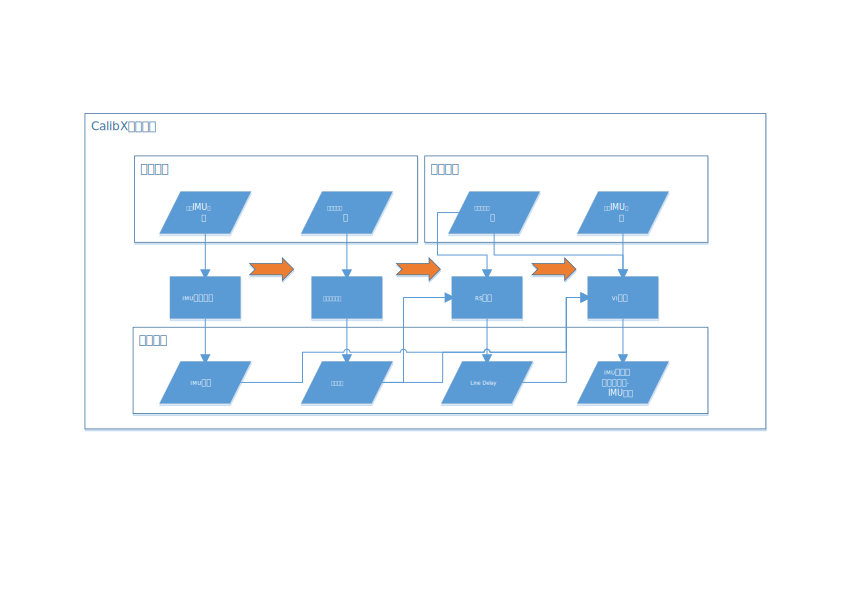
\includegraphics[width=1\textwidth]{figure/target/calibx_framework}
	\caption{CalibX硬件系统}
	\label{fig:calibx_framework}
\end{figure}
目前支持3种相机模型:
\begin{itemize}
	\item Pinhole-brown和pinhole-radtan。主要面向小畸变、小视场角(FOV)的相机。
	\item Pinhole-equidistant。主要面向大畸变、大视场角的相机(FOV $\le $ 180°),主要是广角相机和鱼眼相机。
\end{itemize}
支持4种标定板,如图\ref{fig:calibx-calibration-board}所示。:
\begin{itemize}
	\item 棋盘格。
	\item CircleGrid。
	\item Apriltag。
	\item RandomGrid。
\end{itemize}
\begin{figure}
	\centering
	\begin{minipage}{0.45\linewidth}
		\centering
		\subfigure[棋盘格]{\includegraphics[width=5cm]{figure/target/chessboard}}
		\label{fig:chessboard}
	\end{minipage}\qquad
	\begin{minipage}{0.45\linewidth}
		\centering
		\subfigure[CircleGrid]{\includegraphics[width=5cm]{figure/target/circlegrid}}
		\label{fig:circlegrid}
	\end{minipage}
	\begin{minipage}{0.45\linewidth}
		\centering
		\subfigure[Apriltag]{\includegraphics[width=5cm]{figure/target/apriltag}}
		\label{fig:apriltag}
	\end{minipage}\qquad
	\begin{minipage}{0.45\linewidth}
		\centering
		\subfigure[RandomGrid]{\includegraphics[width=5cm]{figure/target/randomgrid}}
		\label{fig:randomgrid}
	\end{minipage}
	\caption{CalibX标定系统支持的标定板}
	\label{fig:calibx-calibration-board}
\end{figure}
其中,棋盘格和CircleGrid为无局部编码的标定板,Apriltag和RandomGrid为局部编码标定板。\\
CalibX总结有如下优点:
\begin{itemize}
	\item 支持多种相机模型,覆盖普通相机、广角相机和鱼眼相机。
	\item 支持多种类型标定板,支持多块同一类型的、局部编码标定板。比如3块RandomGrid构成的立体直角。
	\item 支持多相机,多相机允许是不同类型相机的组合,如普通相机和鱼眼相机、卷帘曝光相机和全局曝光相机。多相机标定支持重叠视场和无重叠视场两种类型。
	\item 标定速度快。静态标定仅用几张图就能完成标定,标定时间不超过30s。RS标定和联标总计在5分钟内完成。
	\item 高精度。正常情况下,多相机标定基线与设计值的误差在1mm以内,相机与IMU外参平移误差在3mm以内\footnote{标定设备是OPPO无面罩AR眼镜\label{calibration_device}}。
	\item 高重复性精度。与市面上在售的产品\cite{indemind}相比,相机与IMU外参旋转角重复性精度高10倍\textsuperscript{\ref{calibration_device}}!如表\ref{tab:calibx-vs-indemind}所示。
\end{itemize}
\begin{table*}[t]
	\centering
	\caption{CalibX与Indemind标定对比}
	\label{tab:calibx-vs-indemind}
	\begin{tabular}{|c|c|c|c|c|}
		\hline
		方案 & 组别 &  Yaw/° & Pitch/° & Roll/° \\
		\hline
		\multirow{4}{*}{Indemind-双目模组} &1 & -179.521225 & -0.439943 & 0.622170 \\
		\cline{2-5}
		\multirow{4}{*}{} & 2 &-179.602241	&-0.463838	&0.598827 \\
		\cline{2-5}
		\multirow{4}{*}{} & 3 &-179.780491	&-0.662679	&0.404572 \\
		\cline{2-5}
		\multirow{4}{*}{} & STD &0.1326	&0.1223	&0.1195 \\
		\cline{2-5}
		\hline
		\multirow{4}{*}{CalibX-OPPO眼镜} &1 & -89.940266 & 0.209434 & 179.883943 \\
		\cline{2-5}
		\multirow{4}{*}{} & 2 &-89.926987	&0.231154	&179.889317 \\
		\cline{2-5}
		\multirow{4}{*}{} & 3 &-89.919383	&0.258630	&179.889180 \\
		\cline{2-5}
		\multirow{4}{*}{} & STD &0.0106	&0.0247	&0.0031 \\
		\cline{2-5}
		\hline
	\end{tabular}
\end{table*}

\subsection{SLAM最大后验估计模型}
假设移动机器人在时间段$ T = [t_0, t_k] $内,在未知的环境中行走,定义如下的变量:
\begin{itemize}
	\item $ x(t) $: t时刻的机器人状态 
	\item $ u(t) $: t时刻的控制输入
	\item $ m $: 不随时间改变的地图
	\item $ z_i $: $ t_i $时刻的观测,$ 1 \le t_i \le N $ 
	\item $ z_{1:N} $: 所有观测的集合,$ \{z_1, z_2, ..., z_N\} $
\end{itemize}
则连续时间SLAM的后验概率密度函数为: $ p(x(t), m | u(t), z_{1:N}) $。假设机器人初始状态的概率密度$ p(x(t_0)) $已知,则依据贝叶斯分解可得:   
\begin{equation}
	\frac {p(z_{1:N}|x(t), m, u(t))p(x(t), m|u(t))}{p(z_{1:N}|u(t))}
\end{equation}
假设观测值与控制输入独立不相关,则有:
\begin{equation}
	\frac {p(z_{1:N}|x(t), m)p(x(t), m|u(t))}{p(z_{1:N})}
\end{equation}
假设当机器人轨迹x(t)与地图m已知时,测量值之间相互独立,则有:
\begin{equation}
	\frac {p(x(t), m|u(t))\prod_{i=1}^N p(z_i|x(t_i),m)}{p(z_{1:N})}
\end{equation}
最后,假设地图m与机器人轨迹x(t)、控制输入u(t),则有:
\begin{equation}
	\frac {p(m)p(x(t)|u(t))\prod_{i=1}^N p(z_i|x(t_i),m)}{p(z_{1:N})}	
\end{equation}
%%%%%%%%%%%%%%%%%%%%%%%%%%%%%%%%%%%%%%%%%%%%%%%%%%%%%%%%%%%%
\subsubsection{高斯假设}
上述的概率密度均服从高斯分布,此时测量模型的概率分布模型为:
\begin{equation}
	z_i = h(x(t_i),m) + n_i, \quad n_i \sim N(\mu, R_i)	
\end{equation}
其中$ h(\cdot) $是确定性测量函数,$ n_i $表示测量噪声,它服从均值为0,方差为$ R_i $的高斯分布,即:
\begin{equation}
	p(z_i|x(t_i), m) = N(h(x(t_i), m), R_i)	
\end{equation}
同样的,假设地图先验和初始状态均为高斯分布: 
\begin{equation}
	m \sim N(\hat{m}, P_m), \quad x(t_0) \sim N(\hat{x}_0, P_x)	
\end{equation}
在连续时间中,运动模型$ p(x(t)|u(t)) $被认为是连续随机动态系统,通常用差分方程描述:
\begin{equation}
	\dot{x}(t) = f(x(t), u(t)) + w(t)
\end{equation}
其中$ \dot{x}(t) $表示x(t)对时间t的导数,$ f(\cdot) $是确定性函数,$ w(t) $是均值为0的白噪声过程,记为$ \mathcal{G} \mathcal{P} (0, Q\delta(t-t'))$。该白噪声过程的协方差函数为$ Q\delta(t-t') $,其中$ \delta(\cdot) $是狄拉克函数。定义:
\begin{equation}
	e_u(t) := \dot{x}(t) - f(x(t), u(t))
\end{equation}
可以得到:
\begin{equation}
	p(x(t)|u(t)) \propto p(x(t_0))\exp\{-\frac{1}{2}\int_{t_0}^{t_k}e_u(\tau)^T Q^{-1}e_u(\tau) d \tau\}
\end{equation}
%%%%%%%%%%%%%%%%%%%%%%%%%%%%%%%%%%%%%%%%%%%%%%%%%%%%%%%%%%%%
\subsubsection{代价函数}
按照极大似然估计的思想,最大化后验估计的概率,即找到一组最优的$ x(t)^* $和$ m^* $ 是的后验估计的负对数概率最小:
\begin{equation}
	\begin{aligned}
		\{x(t)^*,m^*\} &= \underset{x(t), m}{\arg\min}(-log(p(x(t), m|u(t), z_{1:N}))) \\
		&= \underset{x(t), m}{\arg\min}(c + J_z + J_x + J_m + J_u)  
	\end{aligned}
\end{equation}
其中,c是常量,其它变量定义如下:
\begin{equation}
	\begin{aligned}
		J_z &:= \frac{1}{2}\sum_{i=1}{N}(e_{zi}^T R^{-1} e_{zi}), \quad e_{zi} := z_i-h(x(t_i), m) \\
		J_m &:= \frac{1}{2}e_m^T P_m^{-1} e_m, \quad e_m := m-\hat{m} \\
		J_x &:= \frac{1}{2}e_x^T P_x^{-1} e_x, \quad e_x := x(t_0)-\hat{x}_0 \\
		J_u &:= \frac{1}{2}\int_{t_0}^{t_k} e_u(\tau)^T Q^{-1} e_u(\tau) d \tau 
	\end{aligned}
\end{equation}
去掉常量c,定义代价函数$ J(x(t), m) := J_z + J_x + J_m + J_u $,可以得到:
\begin{equation}
	\{x(t)^*, m^*\} = \underset{x(t), m}{\arg\min}(J(x(t), m))
\end{equation}
%%%%%%%%%%%%%%%%%%%%%%%%%%%%%%%%%%%%%%%%%%%%%%%%%%%%%%%%%%%%
\subsubsection{基础函数}
位姿是从样条中提取出来的,它是有限个基础函数的加权和: 
\begin{equation}
	x(t):=\Phi(t)c, \quad \Phi(t):=[\phi_1(t), ..., \phi_M(t)]
\end{equation}
其中$ x(t) $和$ \phi_j(t) $均是D维向量,而由$ \phi_j(t) $组成的基本矩阵$ \Phi(t) $则是$ D \times M$的矩阵。在此定义下,我们的目的就是估计$ M \times 1 $的参数$ c $。由于位姿使用样条表示,此时它对时间的导数则可以表示为: $\dot{x}(t)=\dot{\Phi}(t)c $对$ J_u $和$ e_u $进行研究:
\begin{equation}
	\begin{aligned}
		e_u(t) &= \dot{x}(t) - f(x(t), u(t)) \\
		&= \dot{\Phi}(t)c-f(\Phi(t)c, u(t)) \\
		&= \dot{\Phi}(t)(\bar{c}+\delta c) - f(\Phi(t)(\bar{c} + \delta c), u(t))\\
		&\approx \dot{\Phi}(t)\bar{c} + \dot{\Phi}(t)\delta c - (f(\Phi(t)\bar{c}, u(t)) + \frac{\partial f}{\partial x} \frac{\partial x}{\partial \delta c} \delta c)\\
		&= \dot{\Phi}(t)\bar{c} - f(\Phi(t)\bar{c}, u(t)) + \dot{\Phi}(t)\delta c - \frac{\partial f}{\partial x} \Phi(t) \delta c\\
		&= \bar{e}_u(t) + E_u(t) \delta c
	\end{aligned}
\end{equation}
其中:
\begin{equation}
	\begin{aligned}
		\bar{e}_u(t)&:=\dot{\Phi}(t)\bar{c}-f(\Phi(t)\bar{c}, u(t))\\
		E_u(t)&:=\dot{\Phi}(t)-\frac{\partial f}{\partial x}\Phi(t)
	\end{aligned}
\end{equation}
此时可得:
\begin{equation}
	\begin{aligned}
		J_u &\approx \frac{1}{2} \int_{t_0}^{t_K}(\bar{e}_u(\tau) + E_u(\tau)\delta c)^T Q^{-1}(\bar{e}_u(\tau) + E_u(\tau)\delta c) d \tau \\
		\frac {\partial J_u}{\partial \delta c}^T &\approx \int_{t_0}^{t_K} E_u(\tau)^T Q^{-1}(\bar{e}_u(\tau) + E_u(\tau)\delta c)d \tau\\
		&= \int_{t_0}^{t_K}E_u(\tau)^T Q^{-1}\bar{e}_u(\tau)d \tau + \int_{t_0}^{t_K}E_u(\tau)^T Q^{-1}E_u(\tau)d \tau \delta c 
	\end{aligned}
\end{equation}
定义:
\begin{equation}
	\begin{aligned}
		A_u &= \int_{t_0}^{t_K}E_u(\tau)^T Q^{-1}E_u(\tau)d \tau \\
		b_u &= \int_{t_0}^{t_K}E_u(\tau)^T Q^{-1}\bar{e}_u(\tau)d \tau
	\end{aligned}
\end{equation}
其中$ A_u $对应高斯牛顿法中的海森(Hessian)矩阵
\subsection{相机-IMU联合标定}
\subsubsection{基于se3求导}
严格上讲,这里并没有使用se3,因为se3的求导形式比较复杂,通常使用另一种位姿表达形式去进行更新。这里定义6DoF的位姿为:
\begin{equation}
	x = \left[
	\begin{matrix}
		t_x \\
		t_y \\
		t_z \\
		\phi_x \\
		\phi_y \\
		\phi_z
	\end{matrix}
	\right]
\end{equation}
其中,$ t = [t_x, t_y, t_y]^T $ 为平移,$ \phi = [\phi_x, \phi_y, \phi_z]^T $ 为旋转(轴角形式),它们与SE3的联系为: 
\begin{equation}
	T = \left[
	\begin{matrix}
		\exp(\phi^{\wedge}) & t\\
		0_{1 \times 3} & 1
	\end{matrix}
	\right]_{4 \times 4}
\end{equation}
记$ T = g(x) $ 和 $ x = g^{-1}(T) $为x与T的映射和逆映射。
$ g(\delta x) * g(x) * p'$
\begin{equation}
	\begin{aligned}
		g(\delta x) * g(x) * p' &= 
		%	
		\left[
		\begin{matrix}
			\exp(\delta \phi) & \delta t \\
			0_{1 \times 3} & 1 
		\end{matrix}
		\right]
		%	
		\left[
		\begin{matrix}
			\exp(\phi) & t \\
			0_{1 \times 3} & 1
		\end{matrix}
		\right]
		%	
		\left[
		\begin{matrix}
			p\\
			1
		\end{matrix}
		\right]\\
		%	
		&= 	\left[
		\begin{matrix}
			\exp(\delta \phi) & \delta t \\
			0_{1 \times 3} & 1 
		\end{matrix}
		\right]
		%	
		\left[
		\begin{matrix}
			Rp+t\\
			1
		\end{matrix}
		\right]\\
		%	
		&= \left[
		\begin{matrix}
			\exp(\delta \phi) (Rp + t) + \delta t \\
			1
		\end{matrix}
		\right]\\
		%	
		\quad \frac {\partial(g(\delta x) * g(x) * p')}{\partial \delta x} &= \left[
		\begin{matrix}
			I_{3 \times 3} & -(Rp + t)^{\wedge} \\
			0 & 0
		\end{matrix}
		\right]
	\end{aligned}
\end{equation}
$ (g(\delta x) * g(x))^{-1} * p'$
\begin{equation}
	\begin{aligned}
		(g(\delta x) * g(x))^{-1} * p' &= g(x)^{-1} * g(\delta x)^{-1} * p' \\
		&= \left[
		\begin{matrix}
			R^T & -R^T t \\
			0 & 1
		\end{matrix}
		\right]
		%	
		\left[
		\begin{matrix}
			\exp(-\delta \phi) & -\exp(-\delta \phi) \delta t \\
			0 & 1
		\end{matrix}
		\right]
		%	
		\left[
		\begin{matrix}
			p\\
			1
		\end{matrix}
		\right]\\
		%	
		&= \left[
		\begin{matrix}
			R^T & -R^T t \\
			0 & 1
		\end{matrix}
		\right]
		%	
		\left[
		\begin{matrix}
			\exp(-\delta \phi) p - \exp(-\delta \phi) \delta t \\
			1
		\end{matrix}
		\right]\\
		%	
		\quad \frac{\partial ((g(\delta x) * g(x))^{-1} * p')}{\partial \delta x} &= \left[
		\begin{matrix}
			R^T & -R^T t \\
			0 & 1
		\end{matrix}
		\right]
		%	
		\left[
		\begin{matrix}
			-I_{3 \times 3} & p^{\wedge} \\
			0 & 0
		\end{matrix}
		\right]\\
		%	
		&= \left[
		\begin{matrix}
			-R^T & R^T p^{\wedge} \\
			0 & 0
		\end{matrix}
		\right]
	\end{aligned}
\end{equation}
设:
\begin{equation}
	\begin{aligned}
		\bar{T} &= \left[
		\begin{matrix}
			\bar{R} & \bar{t} \\
			0 & 1
		\end{matrix}
		\right]\\
		%	
		&= T^{-1}\\
		%	
		&= \left[
		\begin{matrix}
			R^T & -R^T t \\
			0 & 1
		\end{matrix}
		\right]
	\end{aligned}
\end{equation}
则有:
\begin{equation}
	\begin{aligned}
		\frac{\partial ((g(\delta x) * g(x))^{-1} * p')}{\partial \delta x} &=
		\left[
		\begin{matrix}
			-\bar{R} & \bar{R} p^{\wedge}\\
			0 & 0
		\end{matrix}
		\right]\\
		%	
		&= \left[
		\begin{matrix}
			-\bar{R} & \bar{R} p^{\wedge} \bar{R}^T \bar{R} \\
			0 & 0
		\end{matrix}
		\right]\\
		%	
		&= \left[
		\begin{matrix}
			-\bar{R} & (\bar{R} p)^{\wedge} \bar{R} \\
			0 & 0
		\end{matrix}
		\right]\\
		%	
		&= \left[
		\begin{matrix}
			-\bar{R} & (\bar{R}p + \bar{t})^{\wedge} \bar{R} - \bar{t}^{\wedge} \bar{R} \\
			0 & 0
		\end{matrix}
		\right] \\
		%	
		&= -\left[
		\begin{matrix}
			I_{3 \times 3} & -(\bar{R} p + \bar{t})^{\wedge}\\
			0 & 0
		\end{matrix}
		\right]
		%	
		\left[
		\begin{matrix}
			\bar{R} & \bar{t}^{\wedge} \bar{R}\\
			0 & \bar{R}
		\end{matrix}
		\right]
	\end{aligned}
\end{equation}
$ T_a * (g(\delta x) * g(x))^{-1} * p'$
\begin{equation}
	\begin{aligned}
		\frac{\partial (T_a * (g(\delta x) * g(x))^{-1} * p')}{\partial \delta x} &= \left[
		\begin{matrix}
			R_a & t_a \\
			0 & 1
		\end{matrix}
		\right] 
		%	
		(-\left[
		\begin{matrix}
			I_{3 \times 3} & -(\bar{R} p + \bar{t})\\
			0 & 0
		\end{matrix}
		\right]
		%	
		\left[
		\begin{matrix}
			\bar{R} & \bar{t}^{\wedge} \bar{R}\\
			0 & \bar{R}
		\end{matrix}
		\right]) \\
		%	
		&= \left[
		\begin{matrix}
			R_a & -R_a(\bar{R}p + \bar{t})^{\wedge} \\
			0 & 0
		\end{matrix}
		\right]
		(
		-\left[
		\begin{matrix}
			\bar{R} & \bar{t}^{\wedge} \bar{R}\\
			0 & \bar{R}
		\end{matrix}
		\right]
		)\\
		%	
		&\overset{\bar{p}=\bar{R}p + t}{=} \left[
		\begin{matrix}
			R_a & -R_a \bar{p}\\
			0 & 0
		\end{matrix}
		\right]
		(-\left[
		\begin{matrix}
			\bar{R} & \bar{t}^{\wedge} \bar{R}\\
			0 & \bar{R}
		\end{matrix}
		\right]
		)\\
		%	
		&= \left[
		\begin{matrix}
			I_{3 \times 3} & -(R_a \bar{p} + t_a)^{\wedge}\\
			0 & 0
		\end{matrix}
		\right]
		%	
		\left[
		\begin{matrix}
			R_a & t_a^{\wedge}R_a \\
			0 & R_a
		\end{matrix}
		\right]
		%	
		(-\left[
		\begin{matrix}
			\bar{R} & \bar{t}^{\wedge} \bar{R}\\
			0 & \bar{R}
		\end{matrix}
		\right]
		)
	\end{aligned}
\end{equation}
$ g(x + \delta x) * p' $ 
\begin{equation}
	\begin{aligned}
		\left[
		\begin{matrix}
			\exp(\phi + \delta \phi) & t + \delta t \\
			0 & 1
		\end{matrix}
		\right]
		%	
		\left[
		\begin{matrix}
			p\\
			1
		\end{matrix}
		\right] &=
		%	
		\left[
		\begin{matrix}
			\exp(\phi + \delta \phi) p + t + \delta t \\
			1
		\end{matrix}
		\right]\\
		%	
		\frac{\partial(g(x + \delta x) * p')}{\partial \delta x}&=\left[
		\begin{matrix}
			I_{3 \times 3} & -(Rp)^{\wedge} J_l\\
			0 & 0
		\end{matrix}
		\right]\\
		%	
		&= \left[
		\begin{matrix}
			I_{3 \times 3} & -(Rp + t)^{\wedge} J_l + t^{\wedge} J_l\\
			0 & 0
		\end{matrix}
		\right]\\
		%	
		&= \left[
		\begin{matrix}
			I_{3 \times 3} & -(Rp + t)^{\wedge}\\
			0 & 0
		\end{matrix}
		\right]
		%	
		\left[
		\begin{matrix}
			I_{3 \times 3} & t^{\wedge} J_l\\
			0 & J_l
		\end{matrix}
		\right]
	\end{aligned}
\end{equation}
其中$J_l $ 是左雅克比矩阵。
\subsubsection{IMU-相机timeshift估计}
数据融合过程中,需要标定不同传感器之间的time offset. 对于IMU和Camera, 如果需要标定两个传感器之间的time offset, 相机需要采用固定曝光模式.图像打时间戳的方式和设置的曝光时间都会影响timeshift的值. 且对于GS相机和RS相机的影响不完全相同.图像打时间戳的位置会影响标定的timeshift, 下面两图分别显示GS相机(图\ref{fig:gs-timeshift})和RS相机(图\ref{fig:rs-timeshift})图像打时间戳方式对timeshift的影响. 图中, 绿色箭头表示IMU传感器的起始时刻,蓝色箭头表示图像的时间戳打在图像第一行的曝光的起始位置, 红色箭头表示图像的时间戳打在了图像曝光时间的中间, 第二个红色箭头表示图像的时间戳打在了图像中心行的曝光时间的中心位置.
\begin{enumerate}[(1)]
	\item GS相机
	对于GS相机, 图像时间戳打在不同的位置时,timeshift的结果为:
	\begin{itemize}
		\item 图像时间戳打在图像第一行曝光时间的中间, 则timeshift为绿色箭头和蓝色箭头的间隔,即 timeshift = triggering\_delay, 这种情况下, 设置不同的曝光时间不影响 timeshift. 
		\item 图像的时间戳打在图像第一行曝光时间的中间, 则timeshift为绿色箭头和第一行红色箭头的间隔, 即 timeshift = 1/2 * exposure\_time + triggering\_delay, 这种情况下,设置不同的曝光时间, timeshift会不同, 且随曝光时间呈线性变化. 
		\item 图像的时间戳打在图像中心行曝光时间的中间, 则timeshift为绿色箭头和中心行红色箭头的间隔, 即 timeshift = 1/2 * exposure\_time + triggering\_delay, 这种情况下,timeshift和第二种情形一致.	
	\end{itemize}
	\item RS相机
	对于RS相机, 图像时间戳打在不同的位置时,timeshift的结果为:
	\begin{itemize}
		\item 图像时间戳打在图像第一行曝光时间的中间, 则timeshift为绿色箭头和蓝色箭头的间隔,即 timeshift = triggering\_delay, 这种情况下, 设置不同的曝光时间不影响 timeshift.
		\item 图像的时间戳打在图像第一行曝光时间的中间, 则timeshift为绿色箭头和第一行红色箭头的间隔, 即 timeshift = 1/2 * exposure\_time + triggering\_delay, 这种情况下,设置不同的曝光时间, timeshift会不同, 且随曝光时间呈线性变化.
		\item 图像的时间戳打在图像中心行曝光时间的中间, 则timeshift为绿色箭头和中心行红色箭头的间隔, 即 timeshift = 1/2 * exposure\_time + triggering\_delay + 1/2 * image\_height * line\_delay, 这种情况下,timeshift和曝光时间,图像宽度,line\_delay都有关系.
	\end{itemize}
\end{enumerate}
\begin{figure}[H]
	\centering
	\includegraphics[width=1\textwidth]{figure/calibx/gs_imu_cam_timeshift}
	\caption{全局曝光相机timeshift}
	\label{fig:gs-timeshift}
\end{figure}
\begin{figure}[H]
	\centering
	\includegraphics[width=1\textwidth]{figure/calibx/rs_imu_cam_timeshift}
	\caption{卷帘曝光相机timeshift}
	\label{fig:rs-timeshift}
\end{figure}
CalibX 代码中图像时间戳默认打在图像第一行曝光时间的中间, 和 kalibr 一致. Vins-mono代码中图像时间戳默认打在图像中心行曝光时间的中间. 因此, 对于GS相机, CalibX标定的timeshift数值上和Vins-mono一致, 可以将CalibX的标定结果直接传入Vins-mono. 但是, 对于RS相机, CalibX标定的timeshift数值上比Vins-mono少 1/2 * image\_height * line\_delay, 需要在Calibr的标定结果上再加上 1/2 * image\_height * line\_delay , 才能传入Vins-mono. \\
timeshift的标定分为两步, 初始化 + 优化.
\begin{enumerate}[(1)]
	\item 初始化
	利用测量角速度和预测角速度之间的互相关性, 通过求解相关性最大时的时间偏移, 即为 timeshift.
	\begin{itemize}
		\item 根据 pnp 求解的相机位姿以及 IMU-Camera 的外参 Tic, 得到初始化姿态样条. 
		\item 从初始化样条上计算IMU时间戳对应的角速度,即为预测角速度, 计算每个时间戳下预测角速度的模长, 保存到 omega\_predicted\_norm 容器中.
		\item IMU传感器直接测量输出的角速度为测量角速度, 计算每个测量角速度的模长, 保存在 omega\_measured\_norm 容器中.
		\item 对两个容器保存的一维向量进行相关性计算, 得到相关性最大时的timeshift, 即为初始的timeshift值. 如下图\ref{fig:correlation}, 对应的仿真timeshift=0.5 s	
	\end{itemize}
	\item 优化
	对于RS相机, 图像时间戳打在不同的位置时,timeshift的结果为:
	\begin{itemize}
		\item 将timeshift作为优化变量, 带入IMU-Camera标定的目标函数中, 迭代优化timeshift.
		残差方程的构建和td的求解过程可以参考
	\end{itemize}
\end{enumerate}
\begin{figure}[H]
	\centering
	\includegraphics[width=1\textwidth]{figure/calibx/correlation}
	\caption{相机标定流程图}
	\label{fig:correlation}
\end{figure}